Das L"osen von Eigenwertproblemen ist eine Standarddisziplin in der
numerischen linearen Algebra. Die konkrete Problemstellung dabei lautet: Zu gegebenen Matrizen $A,B\in\Cnn$ sollen Paare $(\lambda, x)$ mit $\lambda\in\C$ und $x\in\Co$ gefunden werden, welche
der Gleichung
\[%\begin{equation}\label{chap1:eq:eigenproblem}
Ax = \lambda Bx
\]%\end{equation}

gen"ugen. Solchen \emph{Eigenwertgleichungen} begegnet man in ganz unterschiedlichen Kontexten.
So sind sie beispielsweise bei der Bestimmung von Eigenfrequenzen oder dem Ermitteln von Fixpunkten beim
Rotieren eines Fu"sballs\footnote{Hier wird auf den bekannten
\emph{Satz vom Fu"sball} angespielt. Dieser besagt, dass auf einem Fußball
zwei Punkte existieren, deren Raumkoordinaten zu Spielbeginn und zur Halbzeit
unver"andert sind -- informell formuliert.} ebenso wie beim
Untersuchen des PageRanks\footnote{
Siehe \cite[Abschnitt 2]{page}.
} einer Website von
Bedeutung. Entsprechend strotzt der Kanon von angebotenen numerischen
L"osungsmethoden vor Vielfalt und Virtuosit"at.\footnote{Dies best"atigt sich beispielsweise bei einem Blick in das Inhaltsverzeichnis von \cite{stewart}.}\\

Nun mag der Fall eintreten, da es notwendig wird, lediglich eine Teilmenge
aus der Menge aller Eigenpaare eines gegebenen Problems zu untersuchen:
Man stelle sich vor, man wolle das folgende Bild komprimieren, um den ben"otigten Speicherplatz zu reduzieren.

\begin{figure}[h!]
  \centering
  \resizebox{.4\linewidth}{!}{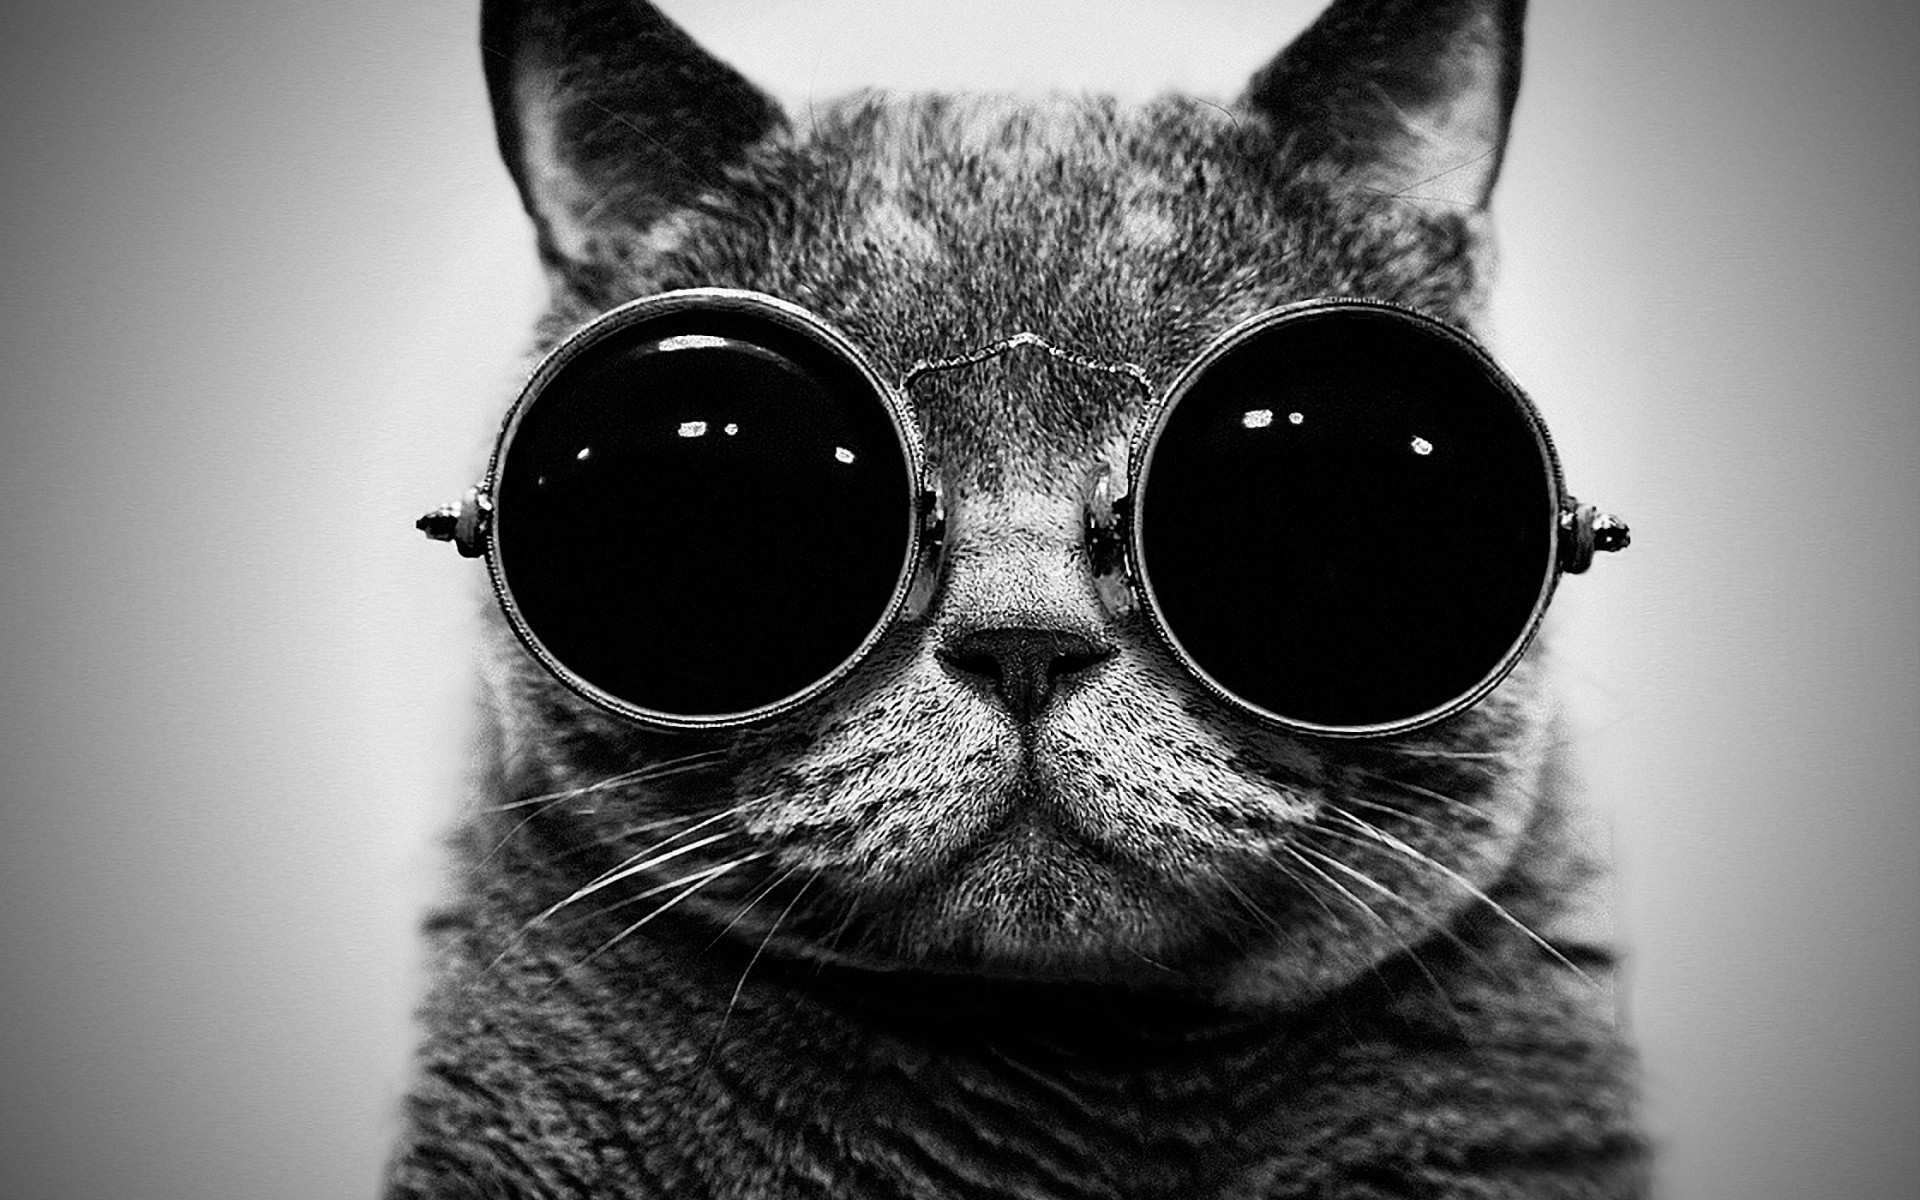
\includegraphics{images/Cat}}
  \caption{\glqq Mind Games of Ozzy\grqq\ von Andy Prokh.}\label{chap1:im:cat}
\end{figure}

%Diese Foto ben"otigt in der Originalgr"o"se einen Speicherplatz von \textcolor{red}{9000mb}.%\footnote{Das Foto aus Abbildung \ref{chap1:im:cat} wurde dabei mit einer \textcolor{red}{tollen Kamera} gemacht.}

Dies l"asst sich beispielsweise mit einer sogenannten \emph{Singul"arwertzerlegung}, welche von Numerikern auch als das \emph{Schweizer Taschenmesser der numerischen linearen Algebra} bezeichnet wird, bewerkstelligen.\\

Da es sich bei Abbildung \ref{chap1:im:cat} um ein Graustufenbild handelt, l"asst sie sich als eine Matrix $M$ auffassen, deren Eintr"age die Grauwerte der einzelnen Pixel repr"asentieren.
Mit einer Singul"arwertzerlegung\footnote{Eine Formulierung ist mit Satz \ref{thm:appTheorems:svd} im Anhang \ref{appTheorems} gegeben.} l"asst sich nun das Bild der Katze durch eine Folge von Matrizen niedrigeren Ranges approximieren.
Man berechnet hierf"ur die Wurzeln der von Null verschiedenen Eigenwerte von $M^H M$ und verwendet diese sogenannten \emph{Singul"arwerte}, um die Matrix $M$ zu rekonstruieren. Wie genau die Singul"arwerte f"ur die Rekonstruktion verwendet werden, soll an dieser Stelle nicht weiter ausgef"uhrt werden.\\

In unserem Beispiel hat $M$ mehr als 700 Singul"arwerte. K"onnen wir uns von einigen Singul"arwerten trennen und dennoch eine akzeptable Bildqualit"at aufrecht erhalten? Und welche Werte wollen wir behalten?\\

Dazu nehmen wir uns die $n$ Singul"arwerte $\sigma_1,\ldots,\sigma_n$ von $M$ her. Ohne Einschr"ankung seien diese so nummeriert, dass $\sigma_1 \ge \ldots \ge \sigma_n$ gilt. Sollte dies nicht der Fall sein, nummerieren wir einfach um.
Nun filtern wir nach eigenen Kriterien Teilmengen aus den Singul"arwerten beziehungsweise den Eigenwerten von $M^H M$ heraus und rekonstruieren mit deren Hilfe die Abbildung \ref{chap1:im:cat}.
Es sei an dieser Stelle darauf hingewiesen, dass die folgendenen Beurteilungen der Bildqualit"at nicht ausschlie"slich mathematisch begr"undet sind.
Die Eindr"ucke entstammen dem pers"onlichen Empfinden des Autors, sowie den Aussagen einer kleinen Testgruppe von Studierenden des Fachs Mathematik.\\

Beginnen wir mit einer mehr oder weniger willk"urlichen Auswahl von Singul"arwerten (SW).

\begin{figure}[h!]
\center
\begin{subfigure}[c]{.3\textwidth}
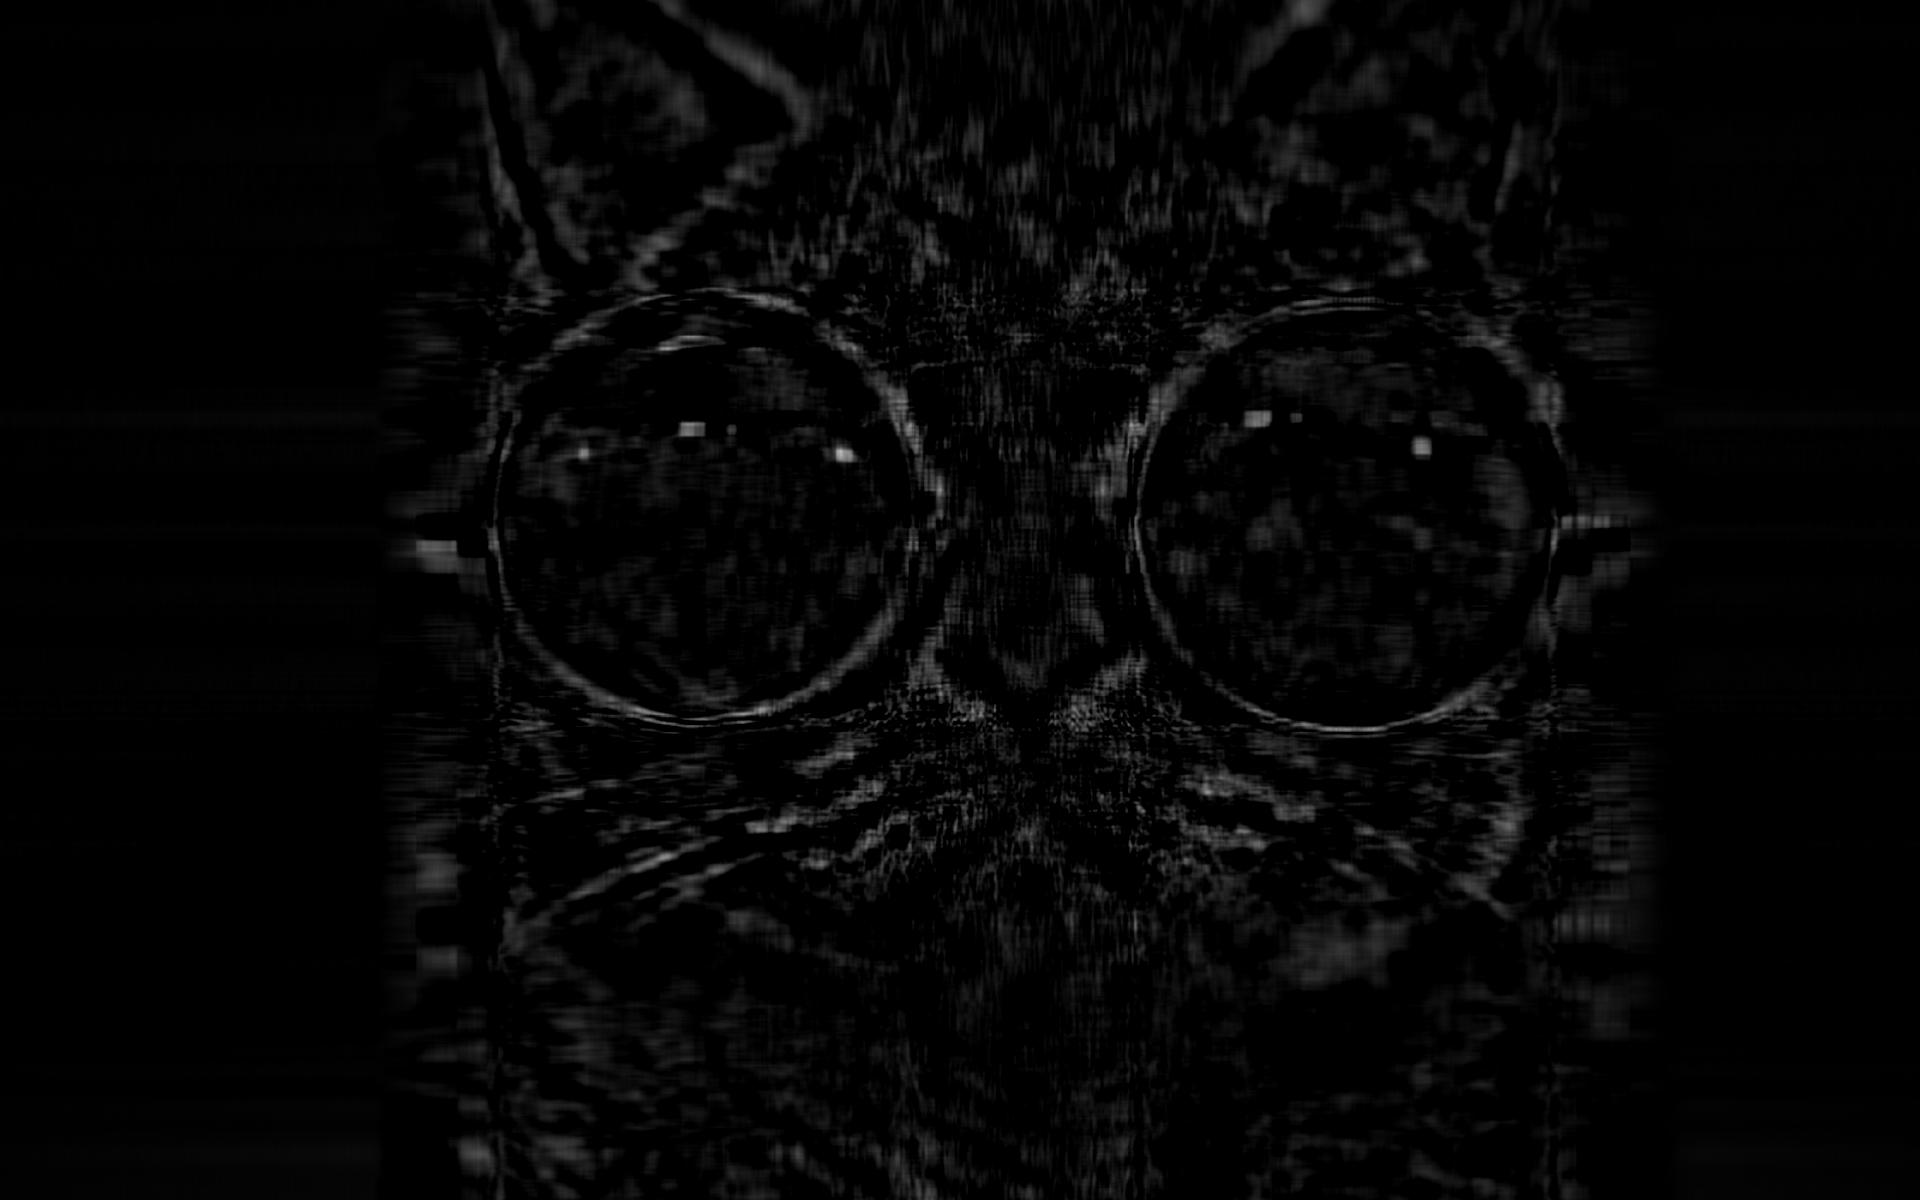
\includegraphics[width=.9\linewidth]{images/Cat10-30}
\subcaption{SW $\sigma_{10},\ldots,\sigma_{30}$.}
\end{subfigure}
\begin{subfigure}[c]{.3\textwidth}
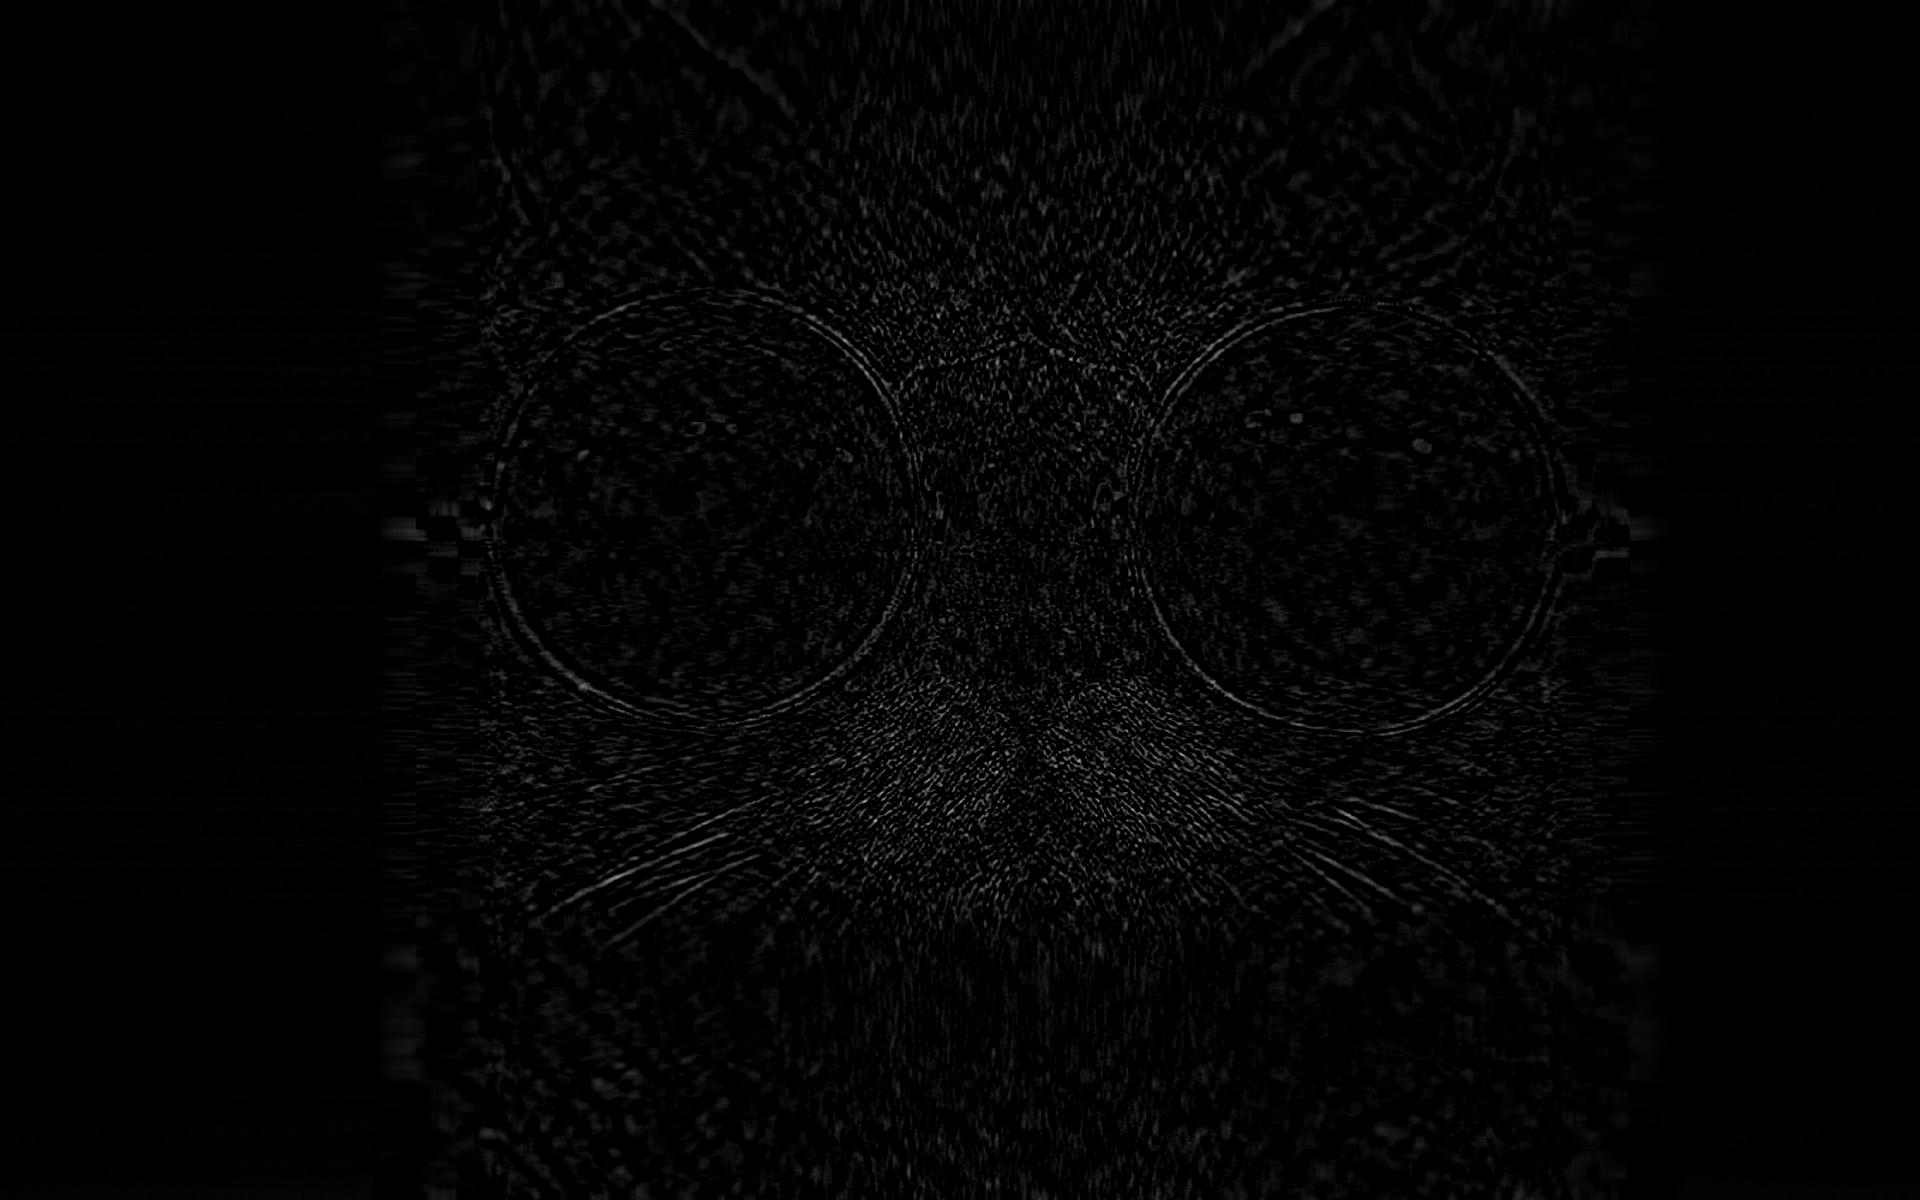
\includegraphics[width=.9\linewidth]{images/Cat40-90}
\subcaption{SW $\sigma_{40},\ldots,\sigma_{90}$.}
\end{subfigure}
\begin{subfigure}[c]{.3\textwidth}
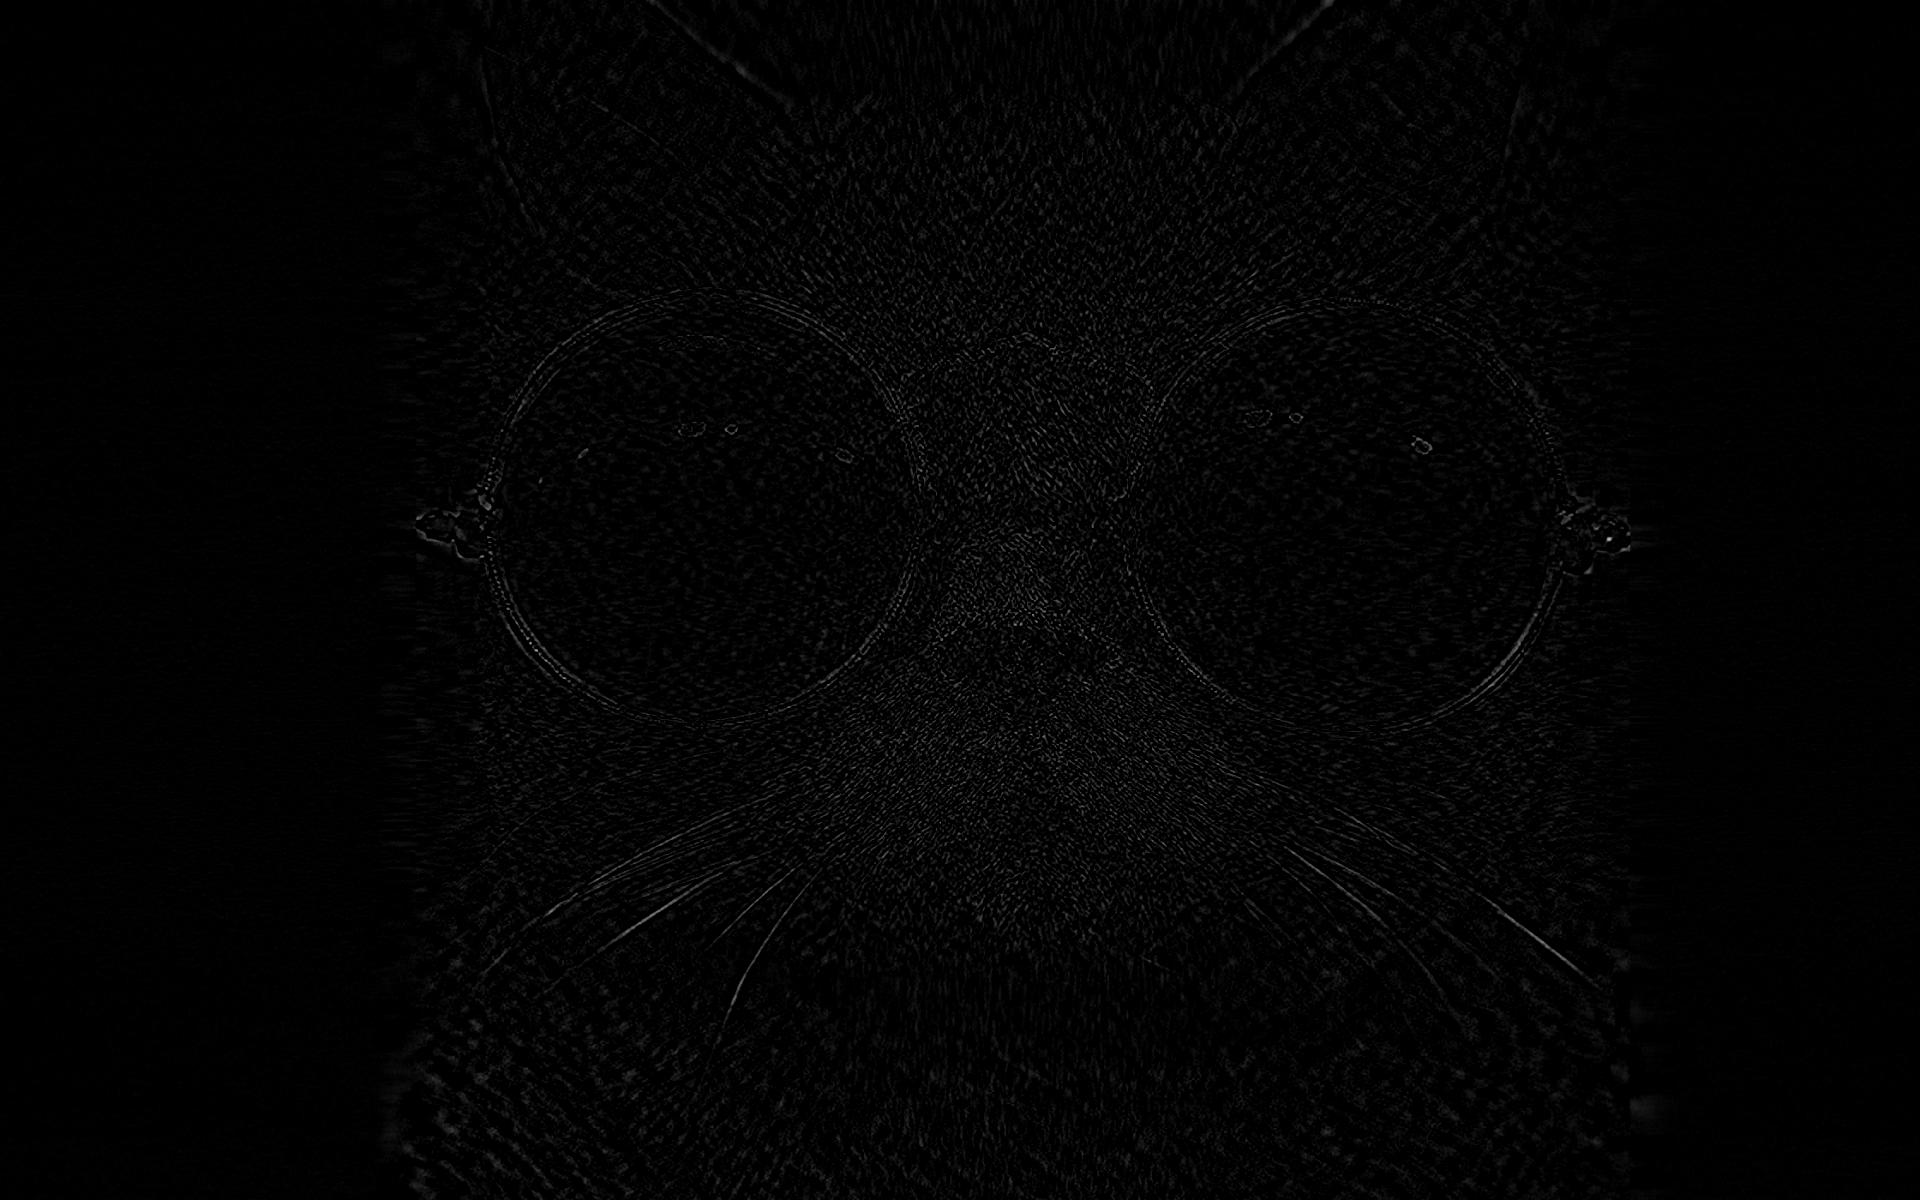
\includegraphics[width=.9\linewidth]{images/Cat100-400}
\subcaption{SW $\sigma_{100},\ldots,\sigma_{400}$.}
\end{subfigure}

\caption{Rekonstruktionsversuch von Abbildung \ref{chap1:im:cat}.}\label{chap1:im:catty}
\end{figure}

Die in Abbildung \ref{chap1:im:catty} gew"ahlten Filtrierungen erscheint etwas ungl"ucklich, da das urspr"ungliche Bild kaum wieder zu erkennen ist.
Daher gestalten wir die Auswahl von SW im n"achsten Rekonstruktionsversuch etwas geschickter und machen uns eine wichtige Konsequenz der Singul"arwertzerlegung zunutze. Sie erm"oglicht es, Matrizen $A_k$ mit der Eigenschaft
\[
\|M - A_k \|_2 = \min_{\substack{B\in\C^{m,n} \\ \text{Rang}(B)=k}} \|M - B\|_2
\]
zu finden.\footnote{Diese Eigenschaft wird in Satz \ref{thm:appTheorems:rang} im Anhang \ref{appTheorems} genauer formuliert.} Dieses Resultat wirkt unmittelbar auf die Bildqualit"at aus, wie in der folgenden Abbildung zu sehen ist.
\newpage

\begin{figure}[h!]
\center
\begin{subfigure}[c]{.3\textwidth}
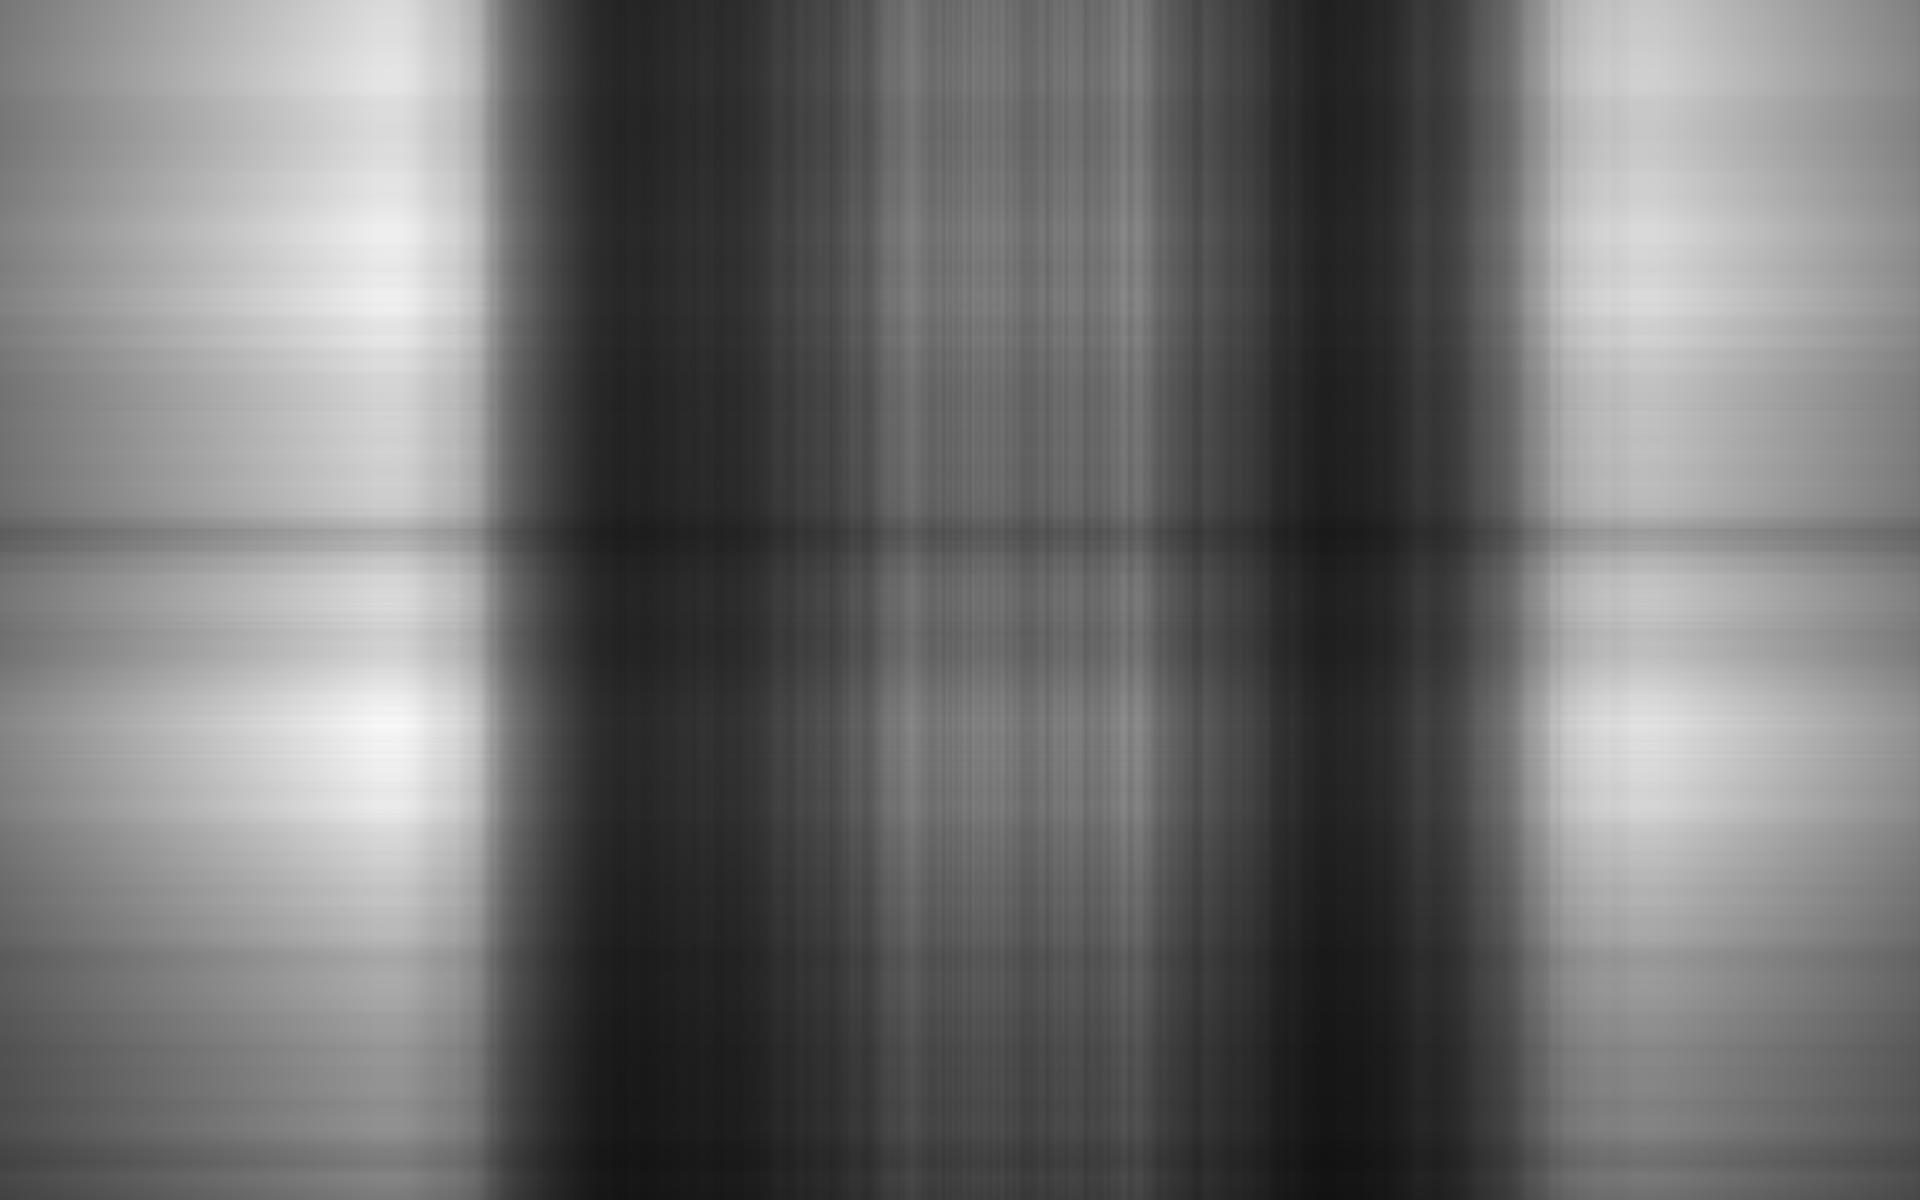
\includegraphics[width=.9\linewidth]{images/Cat1}
\subcaption{SW $\sigma_1$.}
\end{subfigure}
\begin{subfigure}[c]{.3\textwidth}
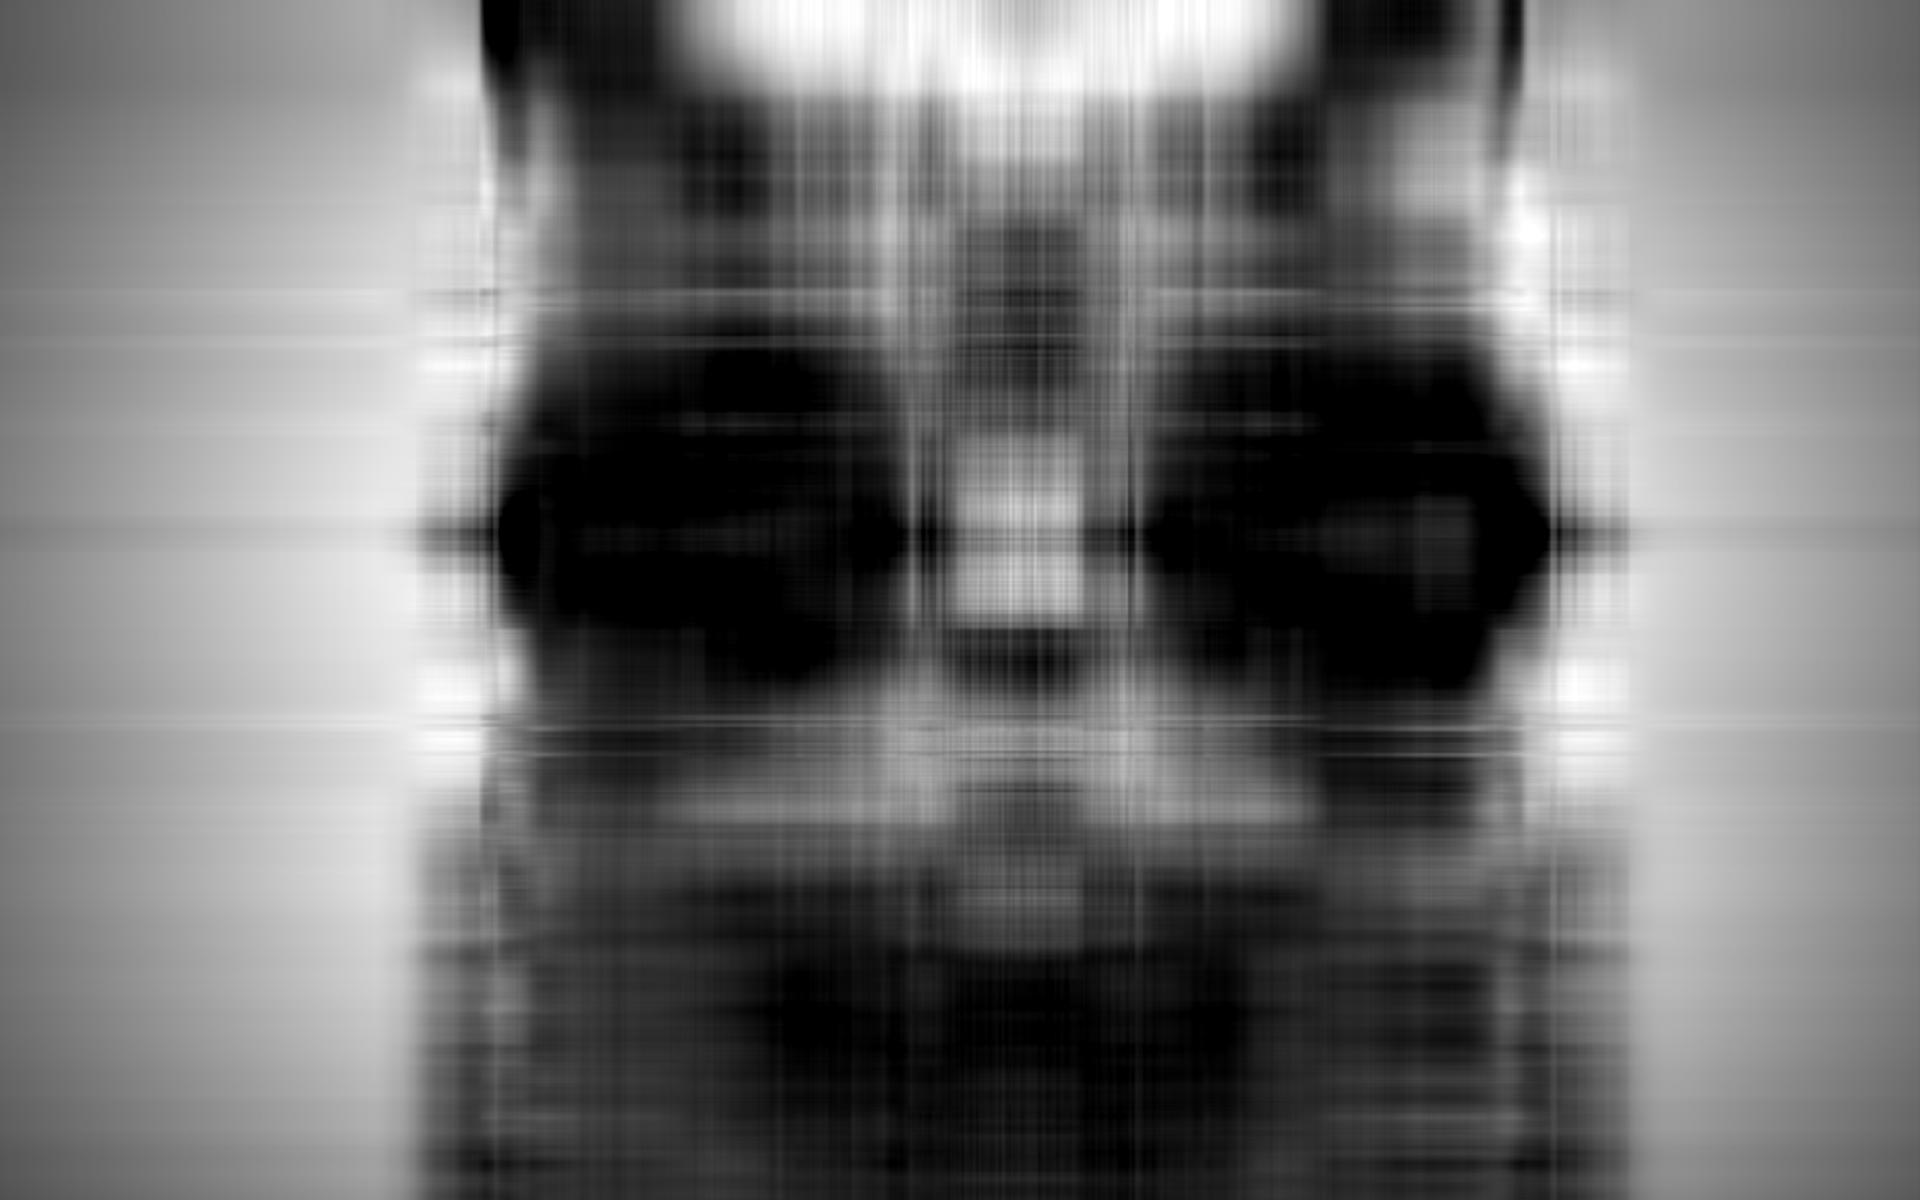
\includegraphics[width=.9\linewidth]{images/Cat5}
\subcaption{SW $\sigma_1,\ldots, \sigma_5$.}
\end{subfigure}
\begin{subfigure}[c]{.3\textwidth}
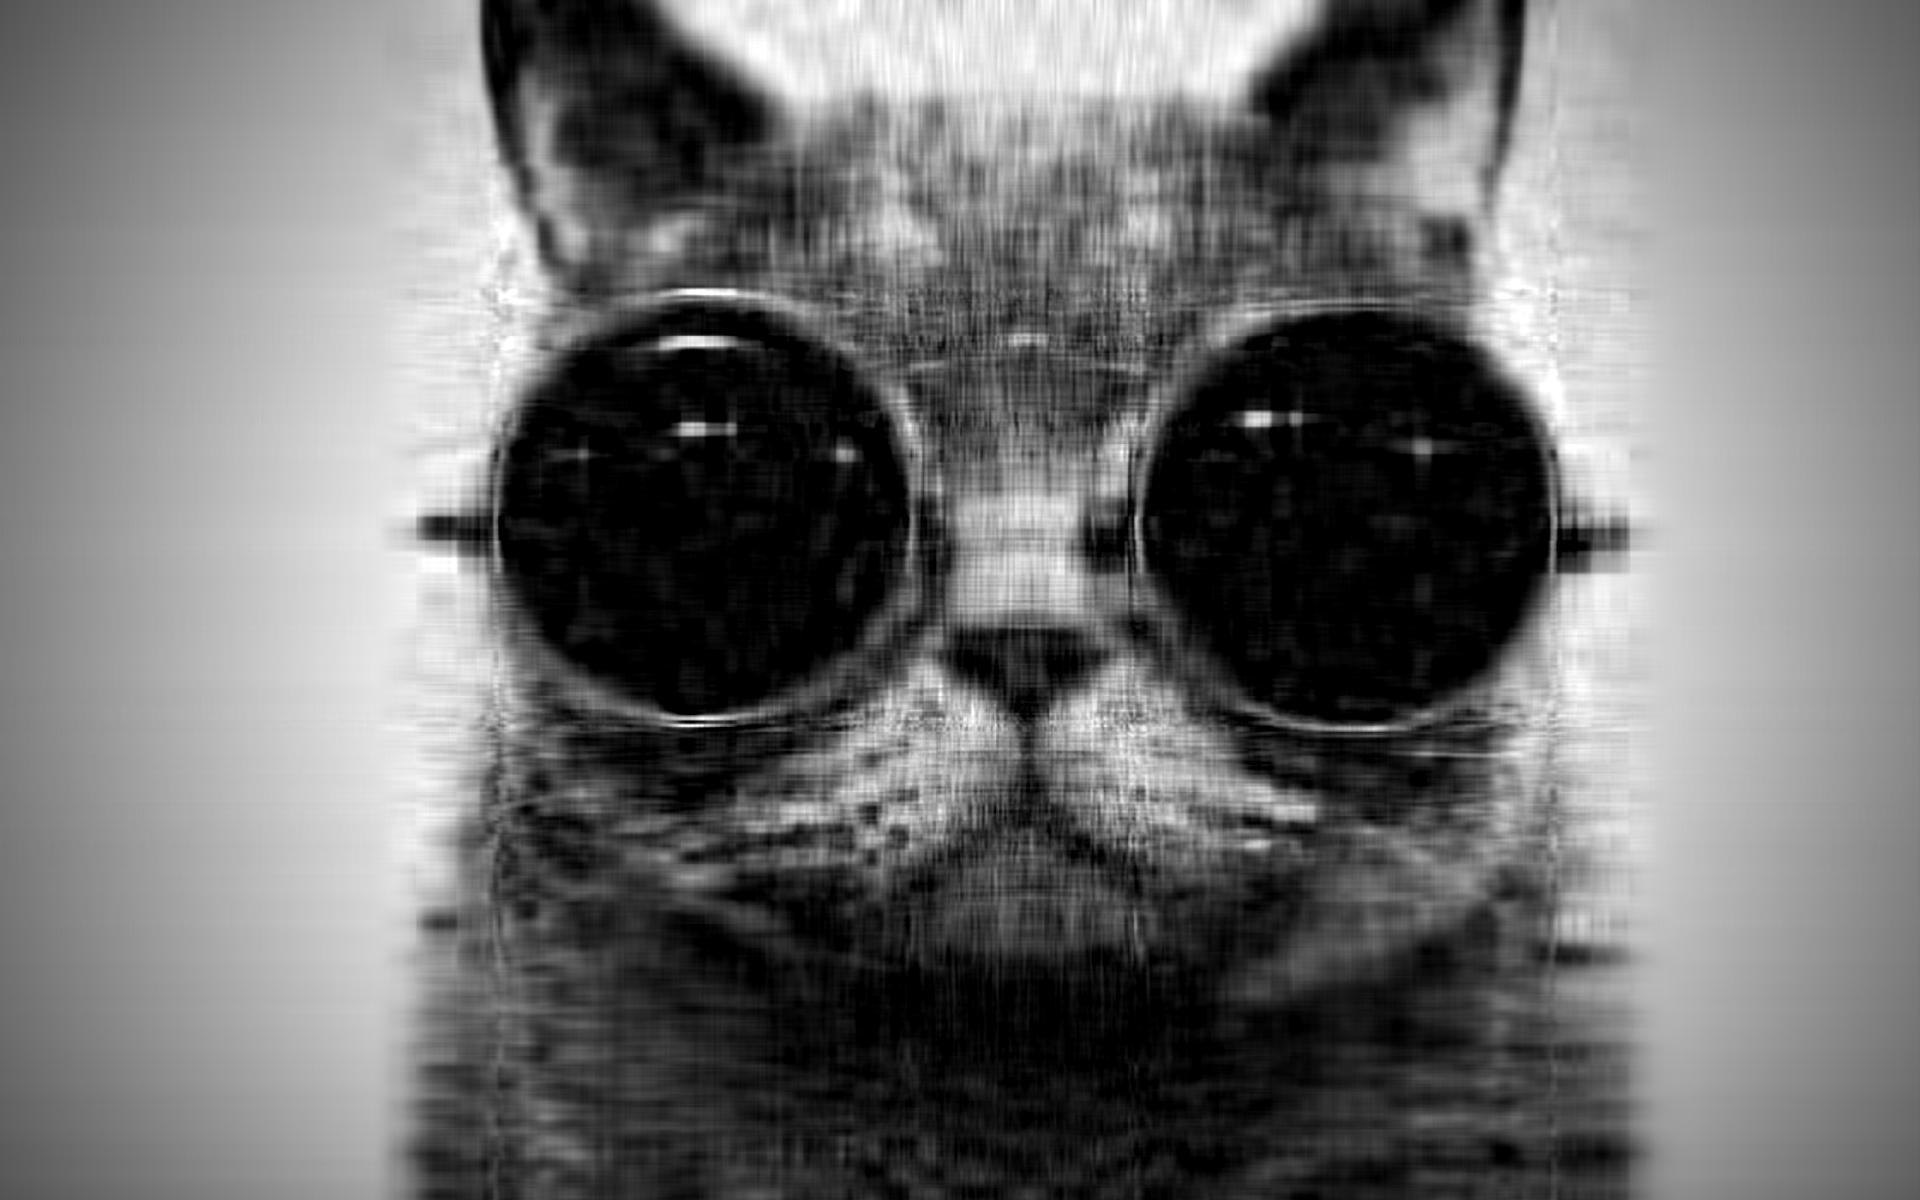
\includegraphics[width=.9\linewidth]{images/Cat20}
\subcaption{SW $\sigma_1,\ldots, \sigma_{20}$.}
\end{subfigure}

\vspace{0.4cm}
\begin{subfigure}[c]{.3\textwidth}
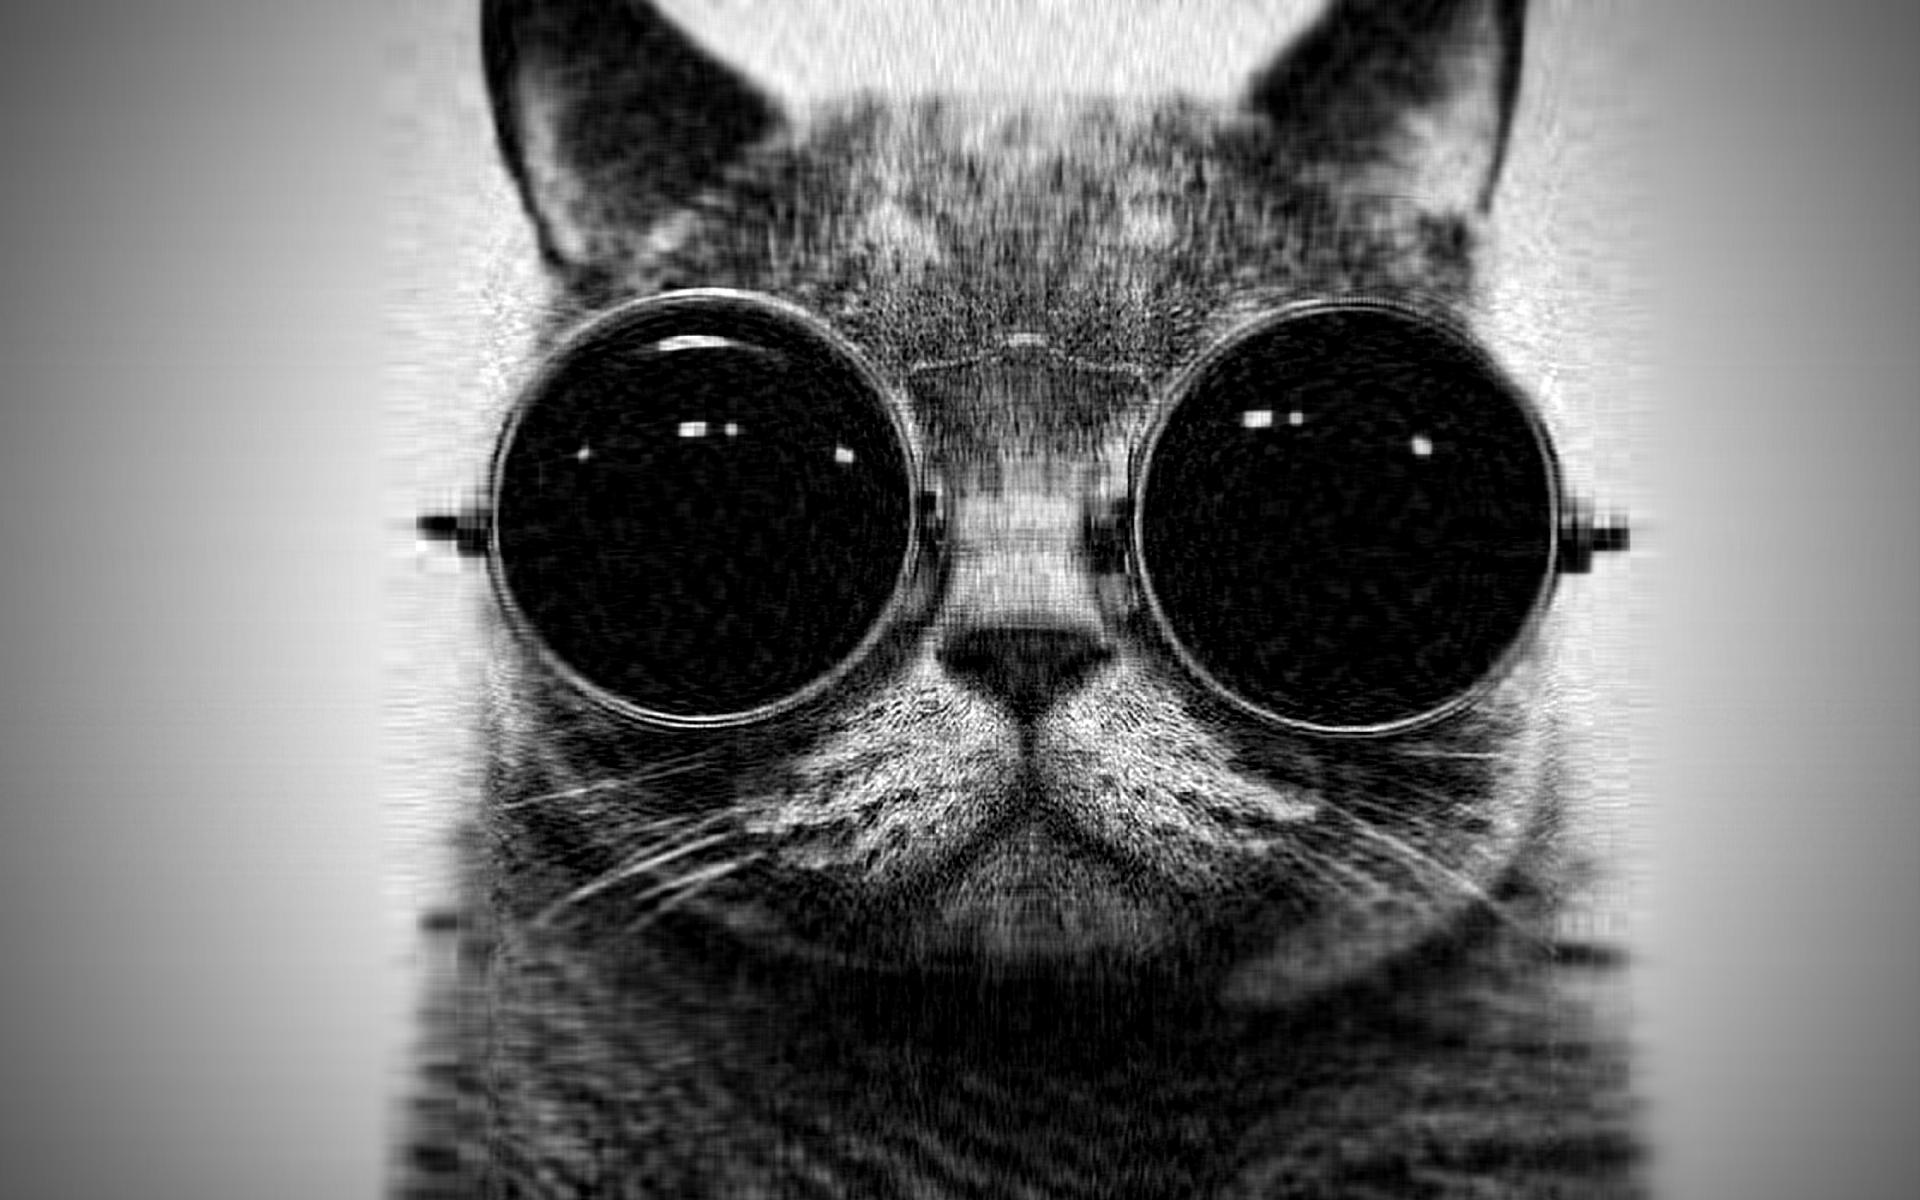
\includegraphics[width=.9\linewidth]{images/Cat50}
\subcaption{SW $\sigma_1,\ldots, \sigma_{50}$.}
\end{subfigure}
\begin{subfigure}[c]{.3\textwidth}
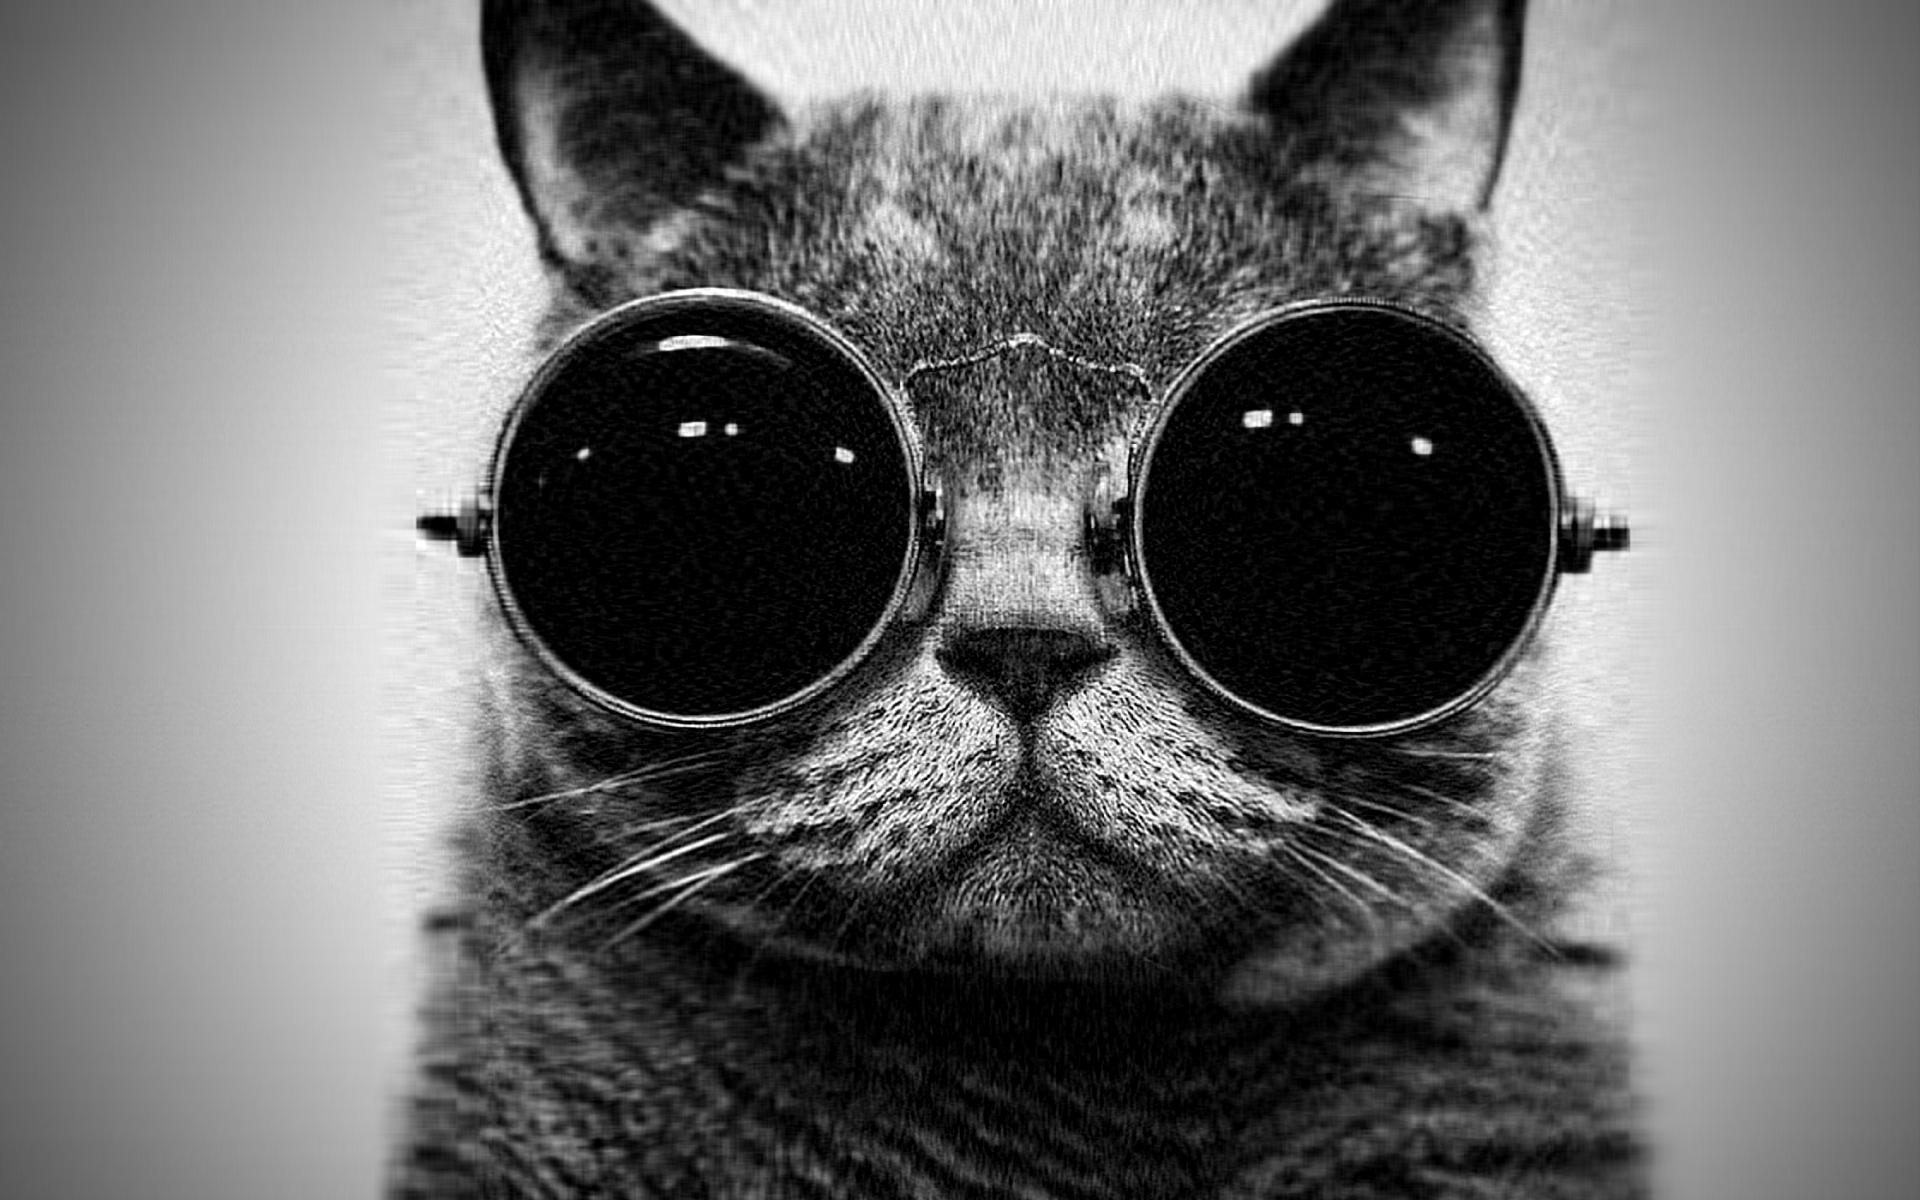
\includegraphics[width=.9\linewidth]{images/Cat100}
\subcaption{SW $\sigma_1,\ldots, \sigma_{100}$.}\label{im:chap1:subE}
\end{subfigure}
\begin{subfigure}[c]{.3\textwidth}
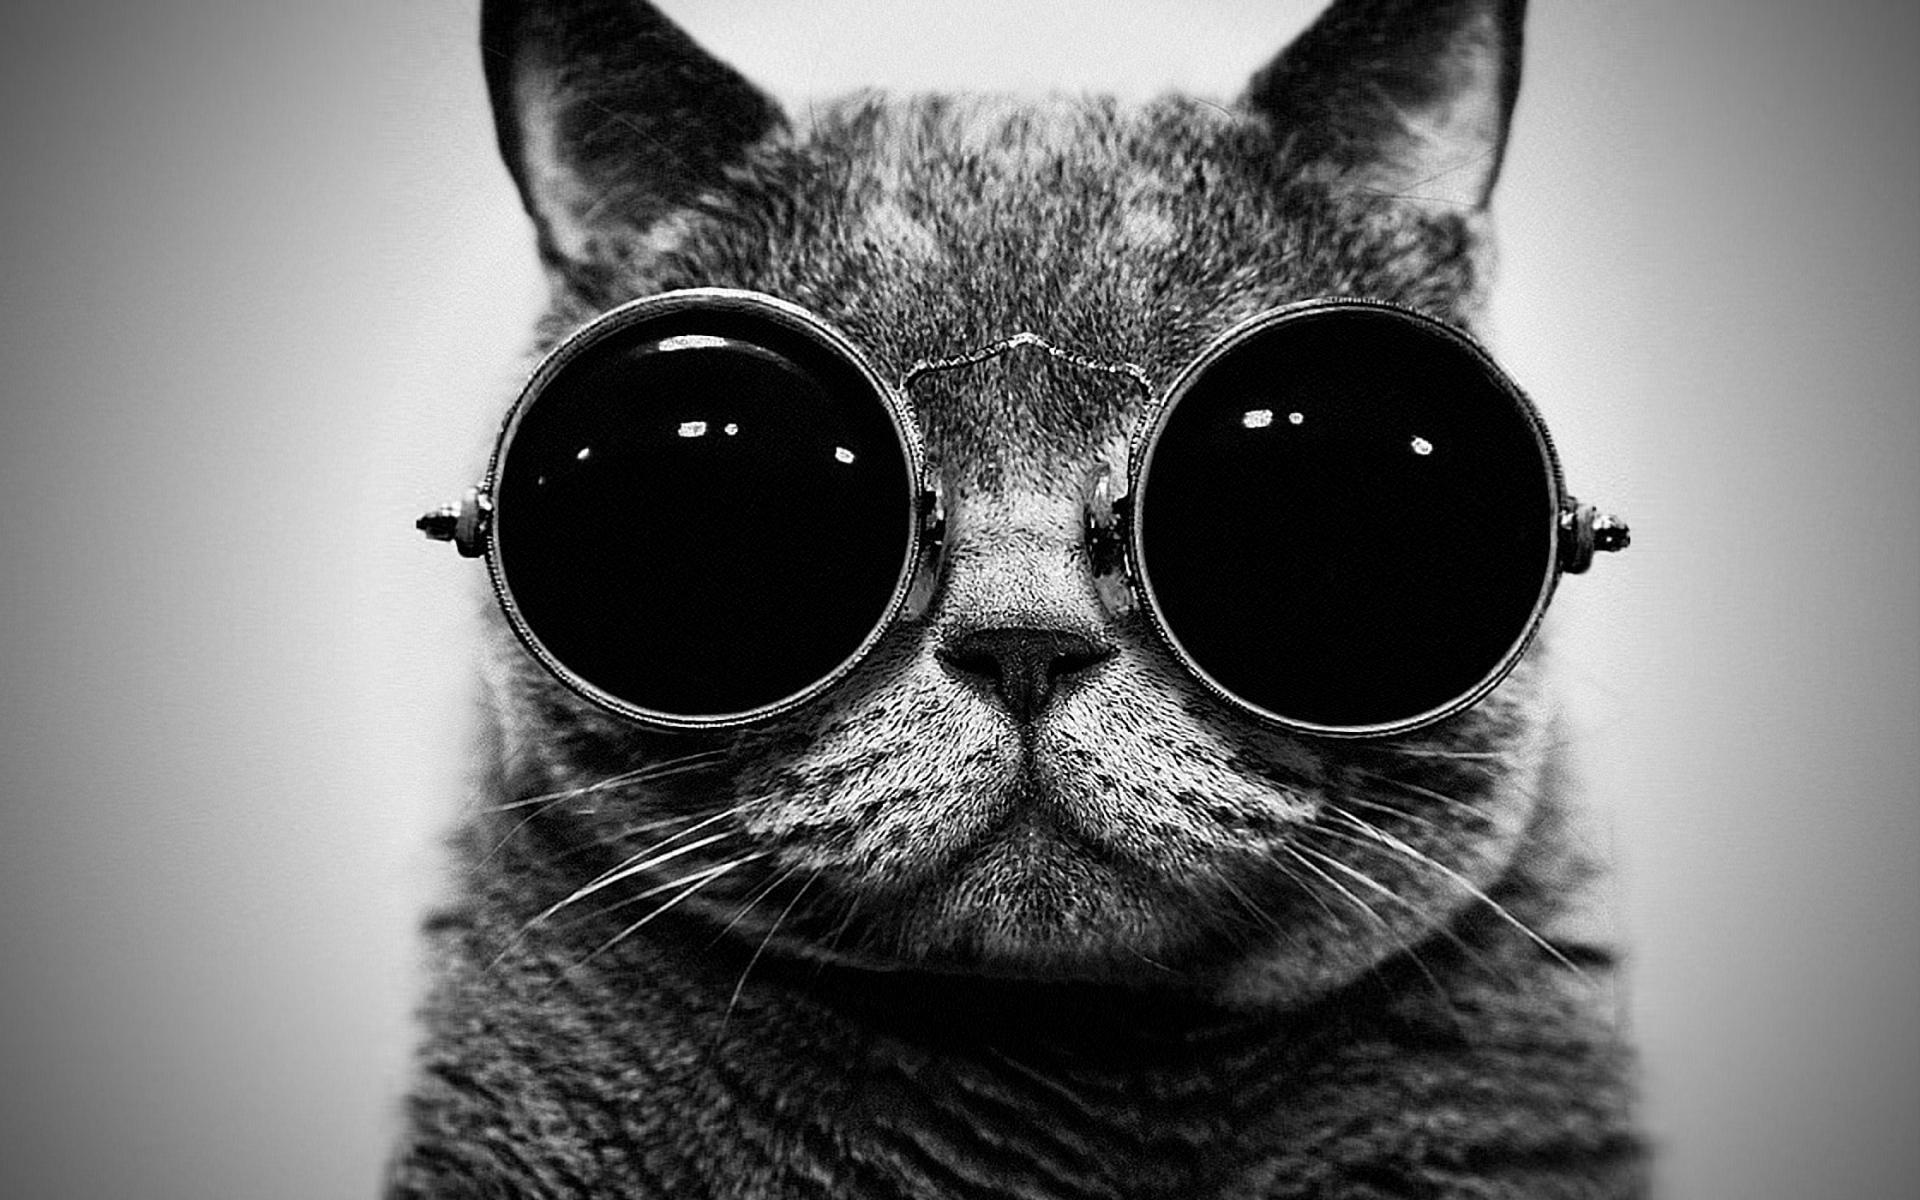
\includegraphics[width=.9\linewidth]{images/Cat300}
\subcaption{SW $\sigma_1,\ldots, \sigma_{300}$.}\label{im:chap1:subF}
\end{subfigure}

\caption{Erneuter Rekonstruktionsversuch von Abbildung \ref{chap1:im:cat}.}
\end{figure}

Dieser Versuch wirkt optisch in der Tat "uberzeugender. Bereits im Bild \ref{im:chap1:subE} ist ein genauer Blick erforderlich, um die Einb"u"sungen bei der Komprimierung zu erkennen.
Bei der Verwendung der ersten 300 SW ist es nahezu unm"oglich, einen Unterschied zum Original festzustellen.
Es ist also zu "uberlegen, ob man sich mit der Qualit"at von \ref{im:chap1:subF} zufrieden geben m"ochte und anstelle von Abbildung \ref{chap1:im:cat} abspeichert.\\

Nun ist das Approximieren von Bildern ein sehr spezieller Fall des Filterns von Eigenwerten und die Berechnung der Singul"arwertzerlegung nicht immer zweckm"a"sig oder m"oglich.
Daher setzt sich diese Arbeit mit Alternativen auseinander, die f"ur Filtrierungen dienlich sind. Dabei werden neben den mathematischen Ideen dieser Alternativen auch M"oglichkeiten der Implementation vorgestellt.\\

Im dritten Kapitel werden zun"achst zwei Methoden pr"asentiert, die als Werkzeuge zum Filtern von Eigenpaaren dienlich sind.
Daran wird sich nach einer kurzen analytischen Illustration dieser Verfahren eine Diskussion anschlie"sen, bei der untersucht wird, wie es um die praktische Umsetzbarkeit der Verfahren bestellt ist.
Wir werden feststellen, dass sich die vorgestellten Algorithmen kombinieren und modifizieren lassen und zu einem Verfahren f"uhren, welches in der Literatur als FEAST-Algorithmus gehandelt wird. Zum Abschluss begeben wir uns in das \glqq Numerik-Labor\grqq\ und werden die Verhaltensweisen der Algorithmen untersuchen.\\

Bevor es konkreter wird, erinnert der folgende Abschnitt an einige mathematische Grundlagen, die als helfende Handreichung das Lesen dieser Schrift mehr zur Freude, als zur Schikane machen soll.

\newpage
\textcolor{white}{bla}
